\documentclass
%[handout]
{beamer}
%\documentclass{beamer}

%%
%%
%%
% From http://tex.stackexchange.com/questions/2072/beamer-navigation-circles-without-subsections
% Solution #2 or 3:
% \usepackage{etoolbox}
% \makeatletter
% % replace the subsection number test with a test that always returns true
% \patchcmd{\slideentry}{\ifnum#2>0}{\ifnum2>0}{}{\@error{unable to patch}}%
% \makeatother
% Solution #1:
\usepackage{remreset}% tiny package containing just the \@removefromreset command
\makeatletter
\@removefromreset{subsection}{section}
\makeatother
\setcounter{subsection}{1}


\usepackage{etex}
\usepackage{pgf}
\usepackage{tikz}
\usepackage{url}
\usepackage{amsmath}
\usepackage{color}
% \definecolor{red}{rgb}{1,0,0}
\usepackage{ulem}
% \usepackage{booktabs}
\usepackage{colortbl,booktabs}
\renewcommand*{\thefootnote}{\fnsymbol{footnote}}
\usepackage{fancybox}
\usepackage[framemethod=TikZ]{mdframed}
\mdfdefinestyle{FactStyle}{%
  outerlinewidth=0.5,
  roundcorner=1pt,
  leftmargin=1cm,
  linecolor=blue,
  outerlinecolor=blue!70!black,
  backgroundcolor=yellow!40
}
\usepackage{cancel}

  \newcommand\Warning{%
    \makebox[2.4em][c]{%
      \makebox[0pt][c]{\raisebox{.2em}{\Large!}}%
      \makebox[0pt][c]{\color{red}\Huge$\bigtriangleup$}}}%

\usepackage{stackengine}
\usepackage{scalerel}
\usepackage{xcolor}
  \newcommand\dangersign[1][2ex]{%
    \renewcommand\stacktype{L}%
    \scaleto{\stackon[1.3pt]{\color{red}$\triangle$}{\tiny !}}{#1}%
  }



\usepackage{dcolumn}
\newcolumntype{d}[1]{D{.}{.}{#1}}

% From
% http://tex.stackexchange.com/questions/109900/how-can-i-box-multiple-aligned-equations
\usepackage{empheq}
\usepackage{tcolorbox}  \newtcbox{\othermathbox}[1][]{%
  nobeforeafter, tcbox raise base, 
  colback=black!10, colframe=red!30, 
  left=1em, top=0.5em, right=1em, bottom=0.5em}

\newcommand\blue{\color{blue}}
\newcommand\red{\color{red}}
\newcommand\green{\color{green!75!black}}
\newcommand\purple{\color{purple}}
\newcommand\bluegreen{\color{blue!75!green}}
\newcommand\orange{\color{orange}}
\newcommand\redgreen{\color{red!50!green}}
\newcommand\grey{\color{black}}
\newcommand\gap{\vspace{.1in}}
\newcommand\nb{${\red\bullet}\ $}
\newcommand\halfgap{\vspace{.05in}}
\newcommand\divideline{\line(1,0){352}}
\usepackage{marvosym} % for \Smiley

\newcommand{\bluealert}[1]{{\blue\textbf{#1}}}

% \usepackage{beamerthemesplit} %Key package for beamer
\usetheme{Singapore}
% \usetheme{Szeged}
% \usetheme{Garfield}
% \usetheme{CambridgeUS}
% \usenavigationsymbolstemplate{} %Gets rid of slide navigation symbols


\setbeamercolor{separation line}{use=structure,bg=structure.fg!50!bg}
% \begin{beamercolorbox}[colsep=0.5pt]
%   {upper separation line foot}
% \end{beamercolorbox}



\makeatletter
\setbeamertemplate{footline}
{
  \leavevmode%
  \hbox{%
% \begin{beamercolorbox}[colsep=0.5pt]
%   {upper separation line foot}
% \end{beamercolorbox}


  \begin{beamercolorbox}[wd=.5\paperwidth,ht=2.25ex,dp=2ex,colsep=0.5pt]%
    {upper separation line foot}
    \usebeamerfont{author in head/foot}%
    \hspace*{2ex}\insertshortdate:\ \insertshorttitle
  \end{beamercolorbox}%
  \begin{beamercolorbox}[wd=.5\paperwidth,ht=2.25ex,dp=2ex,right]{title in head/foot}%
    \usebeamerfont{title in head/foot}
    {\insertshortauthor}\hspace*{2ex}
  \end{beamercolorbox}}%
  % \begin{beamercolorbox}[wd=.333333\paperwidth,ht=2.25ex,dp=2ex,right]{date in head/foot}%
  %   \usebeamerfont{date in head/foot}\insertshortdate{}\hspace*{2em}
  %   \insertframenumber{} / \inserttotalframenumber\hspace*{2ex} 
  % \end{beamercolorbox}%
  \vskip0pt%
}
\makeatother

\usetikzlibrary{decorations.markings}
\usetikzlibrary{arrows}


\title{Final Exam Review}
\author{Peter Garfield, UCSB Mathematics}
\date{March 15, 2017}
%\institute{}


\useinnertheme{default}

\usefonttheme{serif}
% \usecolortheme{rose}
% \usecolortheme{whale}
% \usecolortheme{orchid}
\usecolortheme{crane}
% \usecolortheme{dolphin}


%TEMPLATE
\setbeamertemplate{navigation symbols}{}

\setbeamertemplate{note page}[compress]

\setbeamertemplate{frametitle}{
  \vspace{0.5em}
  % \begin{centering}
  {\huge\blue\textbf{\textmd{\insertframetitle}}}
  \par
  % \end{centering}
}

% From http://tex.stackexchange.com/questions/7032/good-way-to-make-textcircled-numbers:
\newcommand*\circled[1]{\tikz[baseline=(char.base)]{\node[shape=circle,draw,fill=orange,inner sep=1pt] (char) {#1};}} 
% \renewcommand{\labelenumi}{\circled{\textbf{\arabic{enumi}}}}

\let\olddescription\description
\let\oldenddescription\enddescription
\usepackage{enumitem}
\let\description\olddescription
\let\enddescription\oldenddescription

% \usepackage[loadonly]{enumitem}
\setlist[enumerate,1]{label=\colorbox{orange}{\arabic*.},font=\bfseries}
%\setlist[enumerate,2]{label=\colorbox{blue!25}{(\alph*)},font=\bfseries}
% \setlist[enumerate,1]{label=\arabic*.,font=\bfseries}
\setlist[itemize,1]{label=\red$\bullet$}
\setlist[itemize,2]{label=\blue$\bullet$}

\newcommand\answer[1]{\fbox{#1}}
% \renewcommand\answer[1]{}

\newcommand{\antilog}{\operatorname{antilog}}







\title{Welcome to Math 34A!}
\date{March 29, 2022}


\begin{document}
\small

\section{Introduction}
\frame{
  \frametitle{}
  {\Huge{}Welcome To Math 34A!}\\[.5em]

  {\Huge{}Differential Calculus}
  \vfill
  {\Large{}Instructor:}\\
  \ \hspace*{0.2in} Nathan Schley ({\it Sh}+{\it lye}), \url{schley@math.ucsb.edu}\\
  \ \hspace*{0.2in} South Hall 6701
  \\[0.5em]

  {\Large{}Office Hours:}\\
  \ \hspace*{0.2in} T R 11-11:50, T 3:45-4:35 Details on Gauchospace. 
  \bigskip

  \copyright\ 2017-22\ Daryl Cooper, Peter M.\ Garfield, Nathan Schley\\
  Please do not distribute outside of this course.
  \vfill

}

\frame{
  \frametitle{}

  Math 34A is about\ldots

  \begin{itemize}
  \item Problem-solving using reasoning, algebra and arithmetic
  \item Turning English into Math (and vice versa)
  \end{itemize}

  \bigskip
  \pause


  Math 34A is \alert{not}\ about\ldots

  \begin{itemize}
  \item Memorizing formulas
  \item Rote computations
  \end{itemize}
  Here's a blog that explains this point well. \\
  \href{https://mathwithbaddrawings.com/2015/01/21/are-you-a-dish-washing-robot/}{\bf \blue Math with Bad Drawings: Just Memorizing} \\
  Thankfully, we don't make very good robots. 

}


\frame{
  \frametitle{Do You Have An i$>$clicker?}

  A = Yes,\ \ B = No
  \vspace*{2in}
}

\frame{
  \frametitle{Everything Is On GauchoSpace}

  \alert{See \url{https://gauchospace.ucsb.edu/}}
    \begin{itemize}
    \item Syllabus

    \item Homework: 
      \begin{itemize}
      \item On WeBWorK (link on GauchoSpace)
      \item Due each lecture day before the end of the day
      \item First one is due Thursday, Jan 6th!
      \end{itemize}

    %\item Information about discussions and TAs

    \item Dates of midterm exams and final exam.
      \begin{itemize}
      \item First midterm is Jan 25! (\alert{Yikes!})
      \end{itemize}

    \item Grading system

    \item Consider signing up with {\blue CLAS} = {\blue C}ampus {\blue L}earning {\blue A}ssistance {\blue S}ervices -- More info on Gauchocpase. 
    \end{itemize}
    \vspace*{3in}

}

\frame{
  \frametitle{Everything Is On GauchoSpace}

  \alert{See \url{https://gauchospace.ucsb.edu/}}
    \begin{itemize}
%    \item \alert{Great Effort Rule:}\ If you get a grade of C,
%      C$+$ or B$-$, it will be {\blue{}automatically}\ increased to a
%      B, but {\red{}only}\ if you make a great effort.  This means:
%      \begin{itemize}
%      \item Come to all classes (and i$>$click!).
%      \item Come to all discussion sections.
%      \item Do (\alert{seriously attempt})\ all the homework.
%      \item Take all exams.
%      \end{itemize}
%
%      \pause

    \item Purpose of the class: Solving new problems you haven't
      seen before.
      \pause
      \begin{itemize}
      \item Use reasoning, algebra and arithmetic.
      \item This can get \alert{very difficult} at times.
      \item Memorizing formulas is tempting and \alert{seems} easy, but it's actually harder long-term. 
      \item Word problems are the point.
      \end{itemize}
%
%    \end{itemize}
%    \vspace*{3in}
%
%}
%
%
%\frame{
%  \frametitle{Everything Is On GauchoSpace}
%
%  \alert{See \url{https://gauchospace.ucsb.edu/}}
%    \begin{itemize}


   \pause
   \item You should read the textbook!
      \pause
      \begin{itemize}
      \item It's quite good!
      \item These lectures are not just presenting the textbook-- they complement it.
      \item Your homework problems are pulled from the textbook.
      \item To be ready for exams you should follow both the textbook and the lectures.
      \end{itemize}

    \end{itemize}
    \vspace*{3in}

}




\section{Problem-Solving}






\frame{
  \frametitle{Example Puzzle }

  \begin{center}
    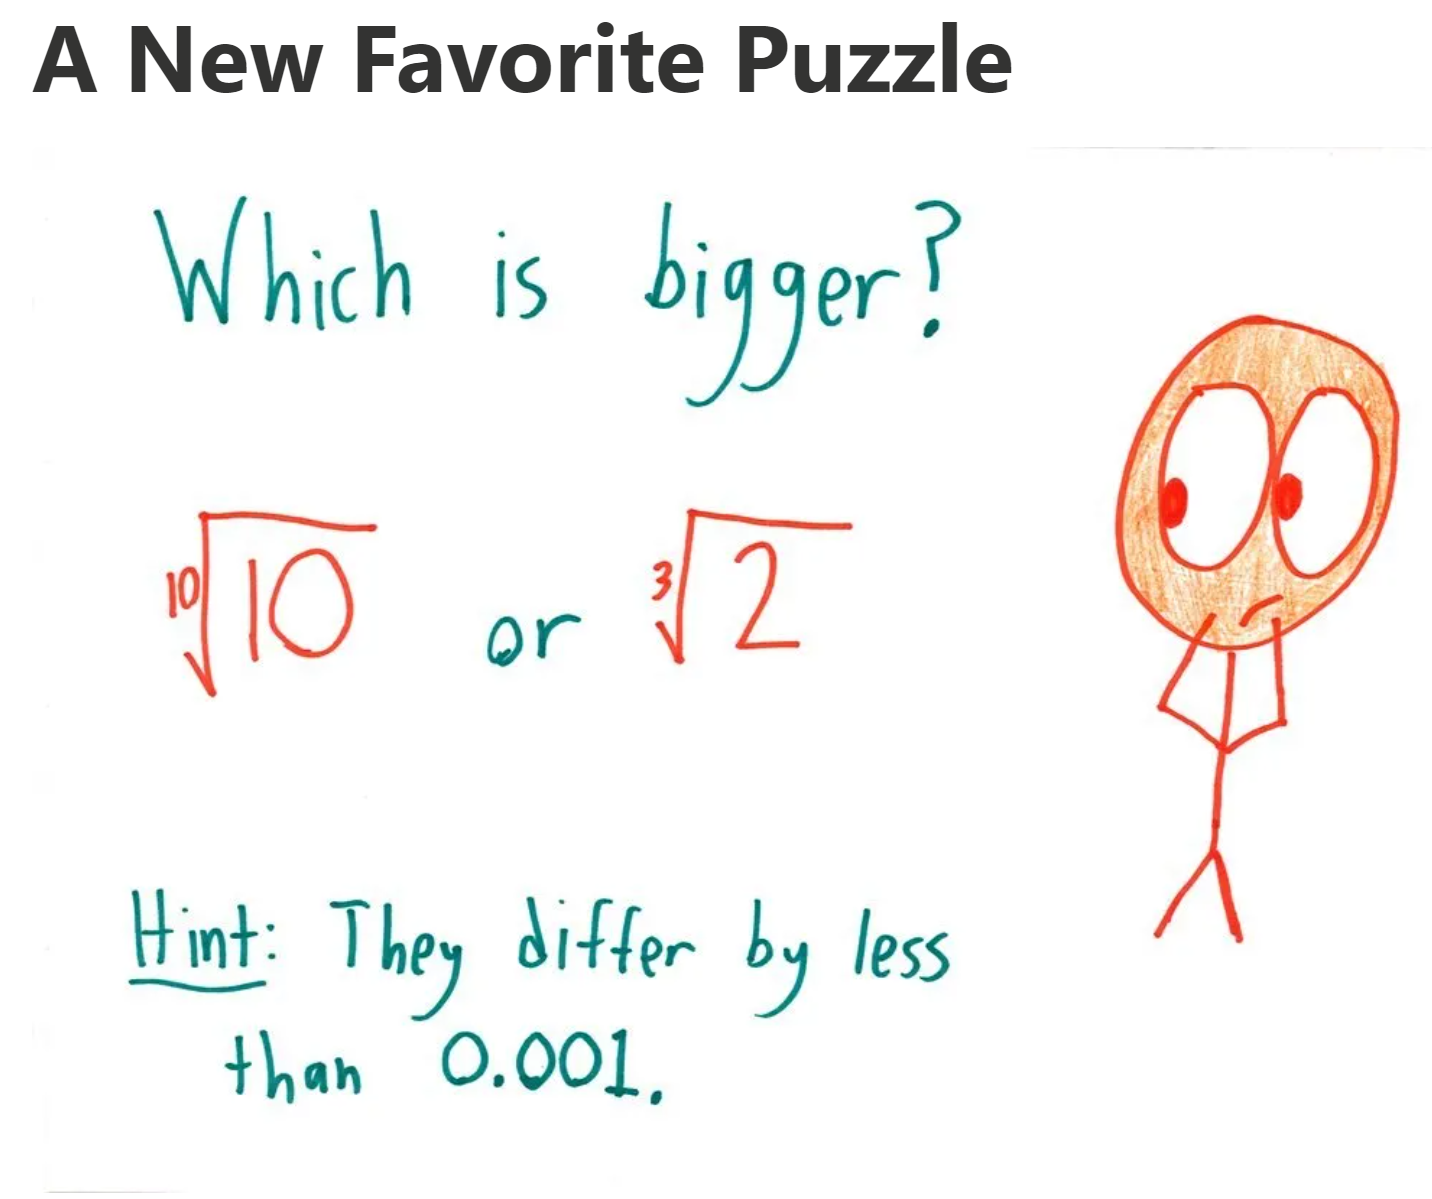
\includegraphics[scale=0.17]{Lecture 1 Puzzle.png}\\
    {\it (From Math with Bad Drawings)} \\
  \end{center}
  \pause 
  \underline{Idea}: The number $2^{10} = 1024$ is often approximated to a ``rounder'' number to convey sizes with computer hardware. 
}






\frame{
  \frametitle{Let's Get Started!}

  \begin{enumerate}
  \item 
    Solve for $x$: \ \ $4x + 7 = 12$
    {\small
      \begin{equation*}
        \text{A} = 3
        \qquad
        \text{B} = 6
        \qquad
        \text{C} = 5/4
        \qquad
        \text{D} = 19/4
        \qquad
        \text{E} = ?
      \end{equation*}
    }
    \pause

    Answer: \answer{C}
    \bigskip
    \pause

  \item Solve for $x$: $ax+b=c$.
    {\small
      \begin{equation*}
        \text{A} = c/a
        \qquad
        \text{B} = bc/a
        \qquad
        \text{C} = (c+b)/a
        \qquad
        \text{D} = c-b/a
        \qquad
        \text{E} = (c-b)/a
      \end{equation*}
    }
    \pause

    Answer: \answer{E}
    \bigskip
  \end{enumerate}

}

\frame{
  \frametitle{More Problems!}

  \begin{enumerate}
    \setcounter{enumi}{2}
  \item 
    Solve for $x$: \ \ $2x + 7 = ax+k$
    {\small
      \begin{equation*}
        \text{A} = (2-k)/(a-7)
        \qquad
        \text{B} = (k-7)/(2-a)
      \end{equation*}
      \begin{equation*}
        \text{C} = (k-7)/(a-2)
        \qquad
        \text{D} = k-7/a-2
        \qquad
        \text{E} = ?
      \end{equation*}
    }
    \pause

    Answer: \answer{B}
    \bigskip
    \pause


    \item Expand: $(1-x)(1+x+x^2)$
      \bigskip\ 
  \end{enumerate}
  \bigskip
  \pause

  \alert{Moral:}\ Parentheses are awesome!

  \vfill

}

\section*{Word Problems}

\frame{
  \frametitle{Word Problems!}

  \begin{enumerate}
    \setcounter{enumi}{3}
  \item The sum of three consecutive numbers is $99$.  What are the
    numbers?
    \bigskip
    \pause

    \alert{Answer:}\ \answer{$32$, $33$, $34$}
    \bigskip
    \pause

  \item Twice one number is three times another number.  The sum of
    the two numbers is $110$.  What are the numbers?  
    \bigskip 
    \pause

    \alert{Answer:}\ \answer{$66$, $44$}
    \pause
    \bigskip

  \item The perimeter of a rectangle is twice its area.  Find a
    formula for the length of the rectangle in terms of its width.
  \bigskip
  \pause

  \alert{Answer:}\ \answer{$L = \frac{W}{W-1}$}

\end{enumerate}

}




\section{Percentages}

\frame{
  \frametitle{Introduction to Percentages}

  \begin{itemize}
    \item cent means hundred
    \item percent means \colorbox{yellow}{per hundred}\ or \colorbox{yellow}{out of one hundred}. 
    \item So $50\%$ means 50 out of 100\pause, or $\frac{50}{100}$\pause, or $.50$
  \end{itemize}
  \pause 

  \begin{empheq}[box=\othermathbox]{align*}
    \text{To convert a fraction to a percentage: multiply by $100\%$}
  \end{empheq}
  \pause

  Questions:
  \begin{enumerate}
  \item What is $3/4$ as $\%$?
    \begin{equation*}
      A=0.75\%
      \quad 
      B = 30\%
      \quad 
      C = 7.5\%
      \quad 
      D = 75\%
      \quad
      \pause
      \answer{D}
    \end{equation*}
    \vspace*{-0.2in}

  \item What is $20\%$ of $30$?
    \begin{equation*}
      A=600
      \quad 
      B = 60
      \quad 
      C =6
      \quad 
      D = 0.6
      \quad
      \pause\answer{C}
    \end{equation*}
  \end{enumerate}
}

\frame{
  \frametitle{You Try It!}

  \begin{enumerate}
    \setcounter{enumi}{2}
  \item   Click A,B,C,D as you do these problems

    \begin{itemize}
    \item[(A)] What is $20\%$ of $x$?
      \bigskip

    \item[(B)] What is $70\%$ as a fraction?
      \bigskip

    \item[(C)] What is $x\%$ of $50$?
      \bigskip


    \item[(D)] What is $\dfrac{x}{x+1}$ as $\%$?
      \bigskip
    \end{itemize}
  \end{enumerate}

  \pause
  Answers: 
  % \begin{equation*}
    (A)\ $x/5$\quad 
    (B)\ $7/10$\quad 
    (C)\ $x/2$\quad 
    (D) $\displaystyle\left(\frac{100x}{x+1}\right)$\%
    \\
  % \end{equation*}
  How many did you get right?
  \begin{equation*}
    A=4 \text{\blue \Large \Smiley} \quad 
    B=3\quad 
    C=2\quad 
    D=1\quad 
    E=\text{\blue \Large \Frowny}
  \end{equation*}

}


\frame{
  \frametitle{Mixing Paint}

  \begin{enumerate}
    \setcounter{enumi}{3}
  \item If I combine {\blue 5} liters of {\blue blue} paint with {\red
      15} liters of {\red red} paint, what percentage of {\red red}
    paint is in the combination?
    \begin{equation*}
      A\ 15\% \quad 
      B\  5\% \quad 
      C\ 75\% \quad 
      D\ 25\% \quad 
      E\ \text{Other} 
      \pause\quad\answer{C}
    \end{equation*}
    \bigskip
    \pause

  \item If I combine {\blue $x$} liters of {\blue blue} paint with {\red
      $y$} liters of {\red red} paint, what percentage of {\blue blue}
    paint is in the combination?
    \begin{equation*}
      A\ \left(\frac{\blue x}{ {\blue x}+{\red y}}\right)\% \quad 
      B\ \left(\frac{\red y}{ {\blue x}+{\red y}}\right)\%\quad 
      C\ \left(\frac{100 {\red y}}{ {\blue x}+{\red y}}\right)  \%
    \end{equation*}
    \begin{equation*}
      D\ \left(\frac{100{\blue x}}{ {\blue x}+{\red y}}\right)  \%\quad 
      E\ \text{Other}\qquad
      \pause\answer{D}    
    \end{equation*}
    \bigskip
  \end{enumerate}

}

\frame{
  \frametitle{One More Problem!}

  \begin{enumerate}
    \setcounter{enumi}{5}
  \item Express $x$\% of $4$ plus $y$\% of $3$ as a percentage of $12$.
    \pause
  \end{enumerate}
  \ \vspace*{1in}

  Idea: Break down the problem into simple steps {\blue in English}.
  Explain what I'm doing {\red to myself}.
  \ \vspace*{1in}
}


\frame{
  \frametitle{That's it. Thanks for being here. }

  \begin{center}
    
\includegraphics[scale=0.4]{stick_together.png}
  \end{center}
}



% \section{Crasher Info}

% \frame{
%   \frametitle{Waitlist / Crashers}

%   \begin{itemize}
%   \item All approval codes are controlled by the Math Department
%     \begin{itemize}
%     \item Before Jan 12:
%       \begin{itemize}
%       \item[\green$\bullet$] Automatically done from waitlist through GOLD. 
%       \item[\green$\bullet$] Approval codes emailed.
%       \item[\green$\bullet$] Approval codes are not currently available.
%       \end{itemize}

%     \item Jan 12 to Jan 28 (last day to add)
%       \begin{itemize}
%       \item[\green$\bullet$] Only students on waitlist and crashing!

%       \item[\green$\bullet$] Approval codes mailed during Jan 18 to Jan 28.

%       \item[\green$\bullet$] You have 24 hours to add.

%       \end{itemize}
%     \end{itemize}      
%     \bigskip

%   \item If you're crashing, please sign my crashers' list!


%   \end{itemize}



% }

\end{document}


%%% Local Variables: 
%%% mode: latex
%%% TeX-master: t
%%% End: 
